\documentclass[tikz,border=8pt]{standalone}
\usepackage{amsmath}
\usetikzlibrary{positioning,arrows.meta}
\definecolor{navy}{HTML}{1D2D50}
\definecolor{cyan}{HTML}{06B6D4}
\definecolor{orange}{HTML}{F59E0B}
\definecolor{green}{HTML}{16A34A}
\begin{document}
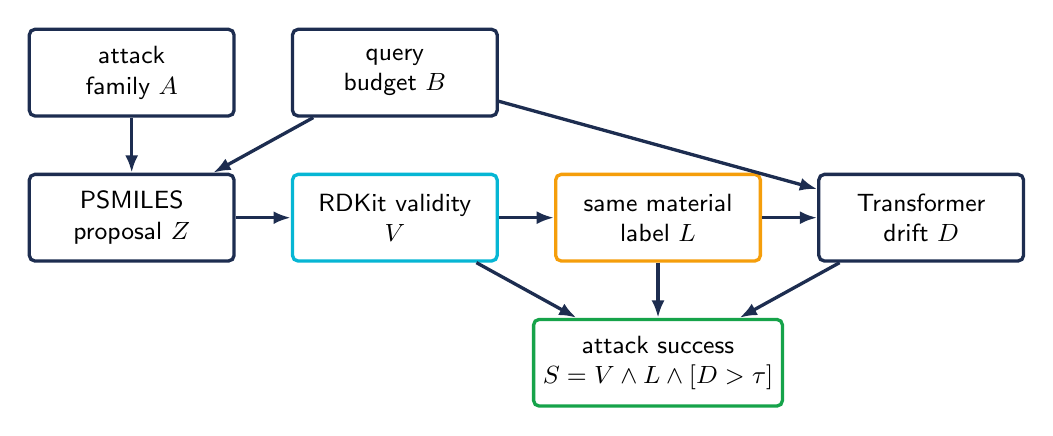
\begin{tikzpicture}[node distance=7mm and 7mm, font=\sffamily\small,
  n/.style={draw=navy,rounded corners=2pt,very thick,fill=white,align=center,minimum width=26mm,minimum height=11mm},
  arr/.style={-{Latex[length=2.2mm]},very thick,draw=navy}]
  \node[n] (a) {attack\\family $A$};
  \node[n,right=of a] (b) {query\\budget $B$};
  \node[n,below=of a] (q) {PSMILES\\proposal $Z$};
  \node[n,right=of q,draw=cyan] (v) {RDKit validity\\$V$};
  \node[n,right=of v,draw=orange] (l) {same material\\label $L$};
  \node[n,right=of l] (d) {Transformer\\drift $D$};
  \node[n,below=of l,draw=green] (s) {attack success\\$S=V\land L\land[D>\tau]$};
  \draw[arr] (a)--(q); \draw[arr] (b)--(q); \draw[arr] (b)--(d);
  \draw[arr] (q)--(v); \draw[arr] (v)--(l); \draw[arr] (l)--(d);
  \draw[arr] (v)--(s); \draw[arr] (l)--(s); \draw[arr] (d)--(s);
\end{tikzpicture}
\end{document}
